%%
%% This is file `sample-manuscript.tex',
%% generated with the docstrip utility.
%%
%% The original source files were:
%%
%% samples.dtx  (with options: `all,proceedings,bibtex,manuscript')
%% 
%% IMPORTANT NOTICE:
%% 
%% For the copyright see the source file.
%% 
%% Any modified versions of this file must be renamed
%% with new filenames distinct from sample-manuscript.tex.
%% 
%% For distribution of the original source see the terms
%% for copying and modification in the file samples.dtx.
%% 
%% This generated file may be distributed as long as the
%% original source files, as listed above, are part of the
%% same distribution. (The sources need not necessarily be
%% in the same archive or directory.)
%%
%%
%% Commands for TeXCount
%TC:macro \cite [option:text,text]
%TC:macro \citep [option:text,text]
%TC:macro \citet [option:text,text]
%TC:envir table 0 1
%TC:envir table* 0 1
%TC:envir tabular [ignore] word
%TC:envir displaymath 0 word
%TC:envir math 0 word
%TC:envir comment 0 0
%%
%% The first command in your LaTeX source must be the \documentclass
%% command.
%%
%% For submission and review of your manuscript please change the
%% command to \documentclass[manuscript, screen, review]{acmart}.
%%
%% When submitting camera ready or to TAPS, please change the command
%% to \documentclass[sigconf]{acmart} or whichever template is required
%% for your publication.
%%
%%
\documentclass[manuscript,screen,review]{acmart}
%%
%% \BibTeX command to typeset BibTeX logo in the docs
\AtBeginDocument{%
  \providecommand\BibTeX{{%
    Bib\TeX}}}

\usepackage{array}
\usepackage{placeins}
\usepackage{algorithm}
\usepackage{algorithmic}
% Prefer vector (PDF) charts when available; fallback to PNG/JPG.
\usepackage{ifthen}
\newcommand{\includebestgraphics}[2][]{%
    % #1 = optional includegraphics options, #2 = base filename without extension
    \IfFileExists{#2.pdf}{%
        \includegraphics[#1]{#2.pdf}%
    }{\IfFileExists{#2.png}{%
        \includegraphics[#1]{#2.png}%
    }{\IfFileExists{#2.jpg}{%
        \includegraphics[#1]{#2.jpg}%
    }{%
        \PackageWarning{includegraphics}{File `#2' not found with .pdf/.png/.jpg extensions}%
    }}}
}
%% Rights management information.  This information is sent to you
%% when you complete the rights form.  These commands have SAMPLE
%% values in them; it is your responsibility as an author to replace
%% the commands and values with those provided to you when you
%% complete the rights form.
\setcopyright{acmlicensed}
\copyrightyear{2018}
\acmYear{2018}
\acmDOI{XXXXXXX.XXXXXXX}
%% These commands are for a PROCEEDINGS abstract or paper.
\acmConference[Conference acronym 'XX]{Make sure to enter the correct
  conference title from your rights confirmation email}{June 03--05,
  2018}{Woodstock, NY}
%%
%%  Uncomment \acmBooktitle if the title of the proceedings is different
%%  from ``Proceedings of ...''!
%%
%%\acmBooktitle{Woodstock '18: ACM Symposium on Neural Gaze Detection,
%%  June 03--05, 2018, Woodstock, NY}
\acmISBN{978-1-4503-XXXX-X/2018/06}


%%
%% Submission ID.
%% Use this when submitting an article to a sponsored event. You'll
%% receive a unique submission ID from the organizers
%% of the event, and this ID should be used as the parameter to this command.
%%\acmSubmissionID{123-A56-BU3}

%%
%% For managing citations, it is recommended to use bibliography
%% files in BibTeX format.
%%
%% You can then either use BibTeX with the ACM-Reference-Format style,
%% or BibLaTeX with the acmnumeric or acmauthoryear sytles, that include
%% support for advanced citation of software artefact from the
%% biblatex-software package, also separately available on CTAN.
%%
%% Look at the sample-*-biblatex.tex files for templates showcasing
%% the biblatex styles.
%%

%%
%% The majority of ACM publications use numbered citations and
%% references.  The command \citestyle{authoryear} switches to the
%% "author year" style.
%%
%% If you are preparing content for an event
%% sponsored by ACM SIGGRAPH, you must use the "author year" style of
%% citations and references.
%% Uncommenting
%% the next command will enable that style.
%%\citestyle{acmauthoryear}


%%
%% end of the preamble, start of the body of the document source.
\begin{document}

%%
%% The "title" command has an optional parameter,
%% allowing the author to define a "short title" to be used in page headers.
\title{Title 3}

%%
%% The "author" command and its associated commands are used to define
%% the authors and their affiliations.
%% Of note is the shared affiliation of the first two authors, and the
%% "authornote" and "authornotemark" commands
%% used to denote shared contribution to the research.
\author{Anne-Marie Rommerdahl}
\affiliation{%
 \institution{SDU}
 \city{Odense}
 \country{Denmark}}
\email{anrom25@student.sdu.dk}

\author{Jeremy Alexander Ramírez Galeotti}
\affiliation{%
 \institution{SDU}
 \city{Odense}
 \country{Denmark}}
\email{jeram25@student.sdu.dk}

\author{Dimitrios Dafnis}
\affiliation{%
 \institution{SDU}
 \city{Odense}
 \country{Denmark}}
\email{didaf25@student.sdu.dk}

\author{Nasifa Akter}
\affiliation{%
 \institution{SDU}
 \city{Copenhagen}
 \country{Denmark}}
\email{naakt23@student.sdu.dk}

\author{Mohammad Hosein Kardouni}
\affiliation{%
 \institution{SDU}
 \city{Odense}
 \country{Denmark}}
\email{mokar25@student.sdu.dk}



%%
%% By default, the full list of authors will be used in the page
%% headers. Often, this list is too long, and will overlap
%% other information printed in the page headers. This command allows
%% the author to define a more concise list
%% of authors' names for this purpose.
\renewcommand{\shortauthors}{}

%%
%% The abstract is a short summary of the work to be presented in the
%% article.



\ccsdesc[500]{Do Not Use This Code~Generate the Correct Terms for Your Paper}
\ccsdesc[300]{Do Not Use This Code~Generate the Correct Terms for Your Paper}
\ccsdesc{Do Not Use This Code~Generate the Correct Terms for Your Paper}
\ccsdesc[100]{Do Not Use This Code~Generate the Correct Terms for Your Paper}

%%
%% Keywords. The author(s) should pick words that accurately describe
%% the work being presented. Separate the keywords with commas.
\keywords{Do, Not, Use, This, Code, Put, the, Correct, Terms, for,
  Your, Paper}

\received{20 February 2007}
\received[revised]{12 March 2009}
\received[accepted]{5 June 2009}

%%
%% This command processes the author and affiliation and title
%% information and builds the first part of the formatted document.
\maketitle

\section{Introduction}


\section{Background and Related Work}
%% ---- Background ----
%% 1 Background abt. reuse. What is it, and why is it important? (anne)
%% 2 What is the current state of 'reuse' for low-code? Anne paragraph (anne)
%% 3 In what ways have different low-code tools tackled 'reuse'? We look at different low-code tools, not just block-based ones. What are the strengths and weaknesses of their approach to reuse? MAKE SURE TO MENTION TOOLS BY NAME! (dimitris)
%% 4 Now we look at block-based tools for robots (for example, scratch, VEXcode GO, OpenRoberta). How do they tackle reuse? (jeremy + Mohamad)
%% 5 Based on the identified weaknesses in current practices for reuse, we propose our own idea (explain how it's gonna work) (Nasifa)

%% ----Re-done intro----
Software reuse is a broad term, that refers to the practice of reusing previously written code, rather than coding from scratch. It is such an important part of software engineering, that one of the ways to measure the quality of software is by its 'Reusability'\cite{SoftwareArchitectureInPractice}, i.e. the degree to which the application or its components can be reused. 
There are multiple benefits to practicing reuse in software engineering. One developer could save time by using another developer's reusable component, rather than coding their own. The developer avoids both the work of writing the syntax and designing the logic of the component. The developer can design their own reusable components, keeping all the logic in one place, which can then be tested thoroughly. However, despite reuse being an important practice in software engineering, there is still a limited focus on this practice when it comes to low-code development platforms (LCDP).

%%--from here: what reuse is there for low-code? What research? IN GENERAL
%%-- Then, what tools? examples of how tools tackle reuse
%%-- Then, what tools for blocks and robots? How do they tackle reuse? What are their strengths/weaknesses/limitations? MAKE SURE TO MENTION BY NAME!!
%%-- Show the tool we'll be working on (what does it do for reuse, and weaknesses).
%%-- Based on all that, what is our idea? What gap is it, we're addressing and how?
%% ---------------------
A study from 2021 studied several low-code platforms (LCPs), in order to identify characteristic features of LCPs. The identified features were presented according to how frequent they occured, with domain-specific reference artifacts being categorized as 'rare'. Most studied systems offered catalogs of "reusable functions or examples of predefined processes", but they were found to be generic, or have a limited scope\cite{LowCodePlatform}. This lack of focus on promoting reuse may impact the so-called 'Citizen Developers', who have little or no coding knowledge, and whom may then miss out on the benefits of reuse. Lin and Weintrop (2021) noted that most existing research on block-based programming focuses on supporting the transition to text-based languages rather than exploring how features within BBP environments \cite{Lin2021Landscape}—such as abstraction or reuse—can enhance learning outcomes.

There have been proposed some ideas on how to promote reuse for LCPs, such as the templating language OSTRICH, developed for model-driven low-code platform OutSystems\cite{OSTRICH}. OSTRICH is designed to assist the end-user in making use of OutSystems' available templates, by abstracting and parameterizing the templates. However, OSTRICH only supports the top nine most used production-ready screen templates, and does not allow the end-user to create and save their own templates, or re-apply a template which they have customized. Another approach focused on enabling the reuse of models, by providing recommendations to the end-user, based on the models stored in a graph acting as a repository. While the graph allows end-users to reuse their own models, there is no mention of guiding the user towards reusing their own models.

%Low code platform tools that focus on reuse
%[x does this, y does that, but a common trend seen in all of them is the almost nonexistent guidance towards using these features. If a user doesnt know/care about reuse, that mentality is never challenged.]
Several popular low-code development platforms (LCDPs) provide different kinds of support for reuse. Webflow\cite{webflow}, a LCDP for responsive websites, offers the ability to create reusable components and UI kits, which can be reused across multiple pages and projects. 
Mendix\cite{mendix} and OutSystems offer even more functionality to support reuse, offering several ways to end-users to share their code with each other, and offering pre-made components. Both of these platforms also utilize AI to enhance reuse. Outsystems provides AI suggestions to spot and create reusable pieces, while Mendix uses AI to suggest the best solutions and components for specific tasks. However, for both of these platforms, the AI suggestions provided are not always accurate to successfully guide the end-user to create custom reusable components ***(How do we know this? What makes it 'accurate'?**).\\
%Mendix\cite{mendix} also offers the ability for end-users to create reusable building blocks, and these can be shared with others. The platform provides AI suggestions to spot and create reusable pieces, empowering even beginners to build complex apps while keeping reuse simple and widespread. This tool does offer guidance for the end-users to create custom reusable components through its AI suggestions, a lot of times these suggestions are not accurate enough*****(HOW do we know whether it's accurate???)****
% Webflow - Despite all of the useful features that this tools has, it does not provide guidance to the end-users to create custom reusable components. % which is the key feature of our project.
% Mendix - This tool does offer guidance for the end-users to create custom reusable components through its AI suggestions, a lot of times these suggestions are not accurate enough (how do we know this??**).
In order to analyze how block-based robotics environments address reuse, 4 representative platforms were compared: mBlock, MakeCode, SPIKE LEGO, VEXcode GO and Open Roberta. The comparison focused on three main dimensions of reuse: structural reuse (through user-defined blocks or functions), social reuse (through sharing or remixing existing projects), and interoperable reuse (through import/export capabilities).
\begin{table}[H]
  \small   
  \caption{Block Based Robotics Environments Reuse Support}
  \label{tab:reuse_support}
  \begin{tabular}{lcccc}
    \toprule
    Platform & Structural Reuse & Social Reuse & Interoperable Reuse & Reuse Support \\
    \midrule
    VEXcode GO    & X & X &  & Medium \\
    mBlock        & X & X & X & Medium \\
    MakeCode      & X & X & X & Medium \\
    Spike Lego    & X &  & X & Low \\
    Open Roberta  &  & X &  & Low \\
    \bottomrule
  \end{tabular}
\end{table}
In this context, “reuse support” represents a scale that measures how effectively each platform facilitates reuse-related features. High reuse support indicates that users can easily create, share, and adapt existing components or projects. Medium reuse support suggests that some reuse mechanisms are available but limited in scope or flexibility. Low reuse support implies that the platform provides only minimal or restricted features to promote reuse.

As shown in Table 1, although these platforms include reusability features, they are quite limited, as none of them provide users with clear guidance on how to use these tools effectively, which restricts their ability to fully leverage them.\\\\
A study by Techapalokul and Tilevich (2019) suggests that supporting mechanisms for reusing smaller, modular pieces of code can enhance programmer productivity, creativity and learning outcomes. 
%Techapalokul and Tilevich (2019) proposed extending the Scratch programming environment with facilities for reusing individual custom blocks to promote procedural abstraction and improve code quality. They observed that while Scratch enables remixing of entire projects, it lacks mechanisms for reusing smaller, modular pieces of code. Their work suggests that supporting such fine-grained code reuse could enhance programmer productivity, creativity, and learning outcomes. Building on this idea, our project applies similar principles within the OpenRoberta environment by automating the detection of duplicate code segments and guiding users toward creating reusable custom blocks.
Adler et al. (2021) introduced a search-based refactoring approach to improve the readability of Scratch programs by automatically applying small code transformations, such as simplifying control structures and splitting long scripts. Their findings demonstrated that automated refactoring can significantly enhance code quality and readability for novice programmers. Building upon this concept, our project applies similar principles in the OpenRoberta environment, focusing on detecting duplicate code segments and guiding users toward creating reusable custom blocks to promote modularity and abstraction.\cite{Adler2021Improving}.

Existing block-based environments provide mechanisms for reuse, but lack intelligent support to help users recognize and apply reuse in practice. To address this gap, our project introduces a guided reuse assistant within the Open Roberta Lab environment.
The tool is designed to help users identify and apply reuse more easily while creating their robot programs. It works by automatically scanning a user’s block-based program to detect repeated code segments in the workspace. The system visually highlights the found duplicates, drawing the user’s attention to patterns that could be simplified.

The tool also offers the functionality to create the custom block for the end-user, by identifying the small differences between the repeated parts—such as numbers, variables, or parameters—and turning these differences into inputs for the new block. The tool automatically replaces all relevant duplicate sequences with the new custom block.

%When repeated blocks are detected, the assistant suggests creating a reusable custom block (function). It then helps the user generate this new block by identifying the small differences between the repeated parts—such as numbers, variables, or parameters—and turning these differences into inputs for the new block. After the user confirms, the system automatically replaces all the repeated sequences with calls to the newly created reusable block.

By combining ideas from procedural abstraction (organizing code into meaningful, reusable parts) and automated refactoring (improving code through intelligent transformations), our tool aims to make block-based programming more structured and efficient.
It encourages users to build programs that are modular and easier to maintain, helps reduce unnecessary repetition, and supports learning by making the concept of reuse clear and hands-on.
%In summary, our work bridges the gap between existing theoretical approaches to software reuse and their real-world application in block-based programming environments. Through this guided and semi-automated approach, we aim to make reuse visible, understandable, and practical for end-users working in Open Roberta.
\section{Study Design}
\label{sec:study_design}

Following the Design Science methodology, our study is structured into three main phases: problem investigation to define goals, treatment design to specify the artifact requirements, and treatment validation to assess the artifact's performance in a controlled environment.

\subsection{Problem Investigation}
\label{subsec:prob_investigation}

\subsubsection{Problem Context and Motivation}

End-user development (EUD) for collaborative robots (cobots) presents unique challenges, particularly for users without formal programming training. In domains such as chemistry laboratories, educational robotics, and industrial settings, end-users need to program 
robots to perform specific tasks but often lack the software engineering knowledge to write maintainable, well-structured code.
In the domain of Chemistry, one of the most relevant and important tasks is performing experiments in labs in order to test a hypothesis, or to aid in the understanding of how chemicals react. 
Robots can be used in chemistry labs to automate experiments with great effect, as many experiments involve steps that are repetitive, and susceptible to human error, such as a step being overlooked, instructions being misread, etc. Automation of menial tasks will leave the chemists with more time for other work, and also comes with the added bonus of chemists not having to handle dangerous chemicals. 
One critical challenge in EUD is code reuse. Users frequently create repetitive code because they struggle to recognize duplicate patterns, lack knowledge about abstraction mechanisms, or find existing tools too complex to use effectively. This problem manifests in several ways: programs become unnecessarily long and difficult to maintain and small changes require modifications in multiple locations, increasing the risk of errors. 
Several  visual programming environments, like OpenRoberta Lab, don't provide assistance in identifying when code should be reused or how to extract repeated sequences into reusable components. As lab work in chemistry involves many repetitive tasks, these challenges can easily become an obstacle for the chemists, which may turn them away from using cobots, as the inconvenience outweighs the benefits.

\subsubsection{Stakeholder Analysis}

Chemists and lab technicians who use cobots for repetitive tasks such as sample preparation, dispensing, mixing, and quality control procedures. 
They possess deep domain expertise in chemistry but limited programming knowledge, often creating long, repetitive programs that become difficult to maintain when adapting experimental protocols. 
Their primary need is to quickly create and modify robot programs without becoming programming experts.


\subsection{Treatment Design}
\label{subsec:treatment_design}

To address the problem of code reuse in EUD for cobots, we have derived a set of requirements designed to contribute to the chemist's goal of creating maintainable and reusable robot programs.
Functionally, the artifact must be capable of automatically detecting duplicate or similar block sequences and visually highlighting these duplications within the user's workspace.
These requirements are necessarry to help the end-user recognize opportunities for reuse, that would otherwise go unnoticed. Once detected, the system must suggest the creation of reusable custom blocks, allowing the user to accept or reject these suggestions.
These signals are important, as they give the end-user control over the reuse process, allowing them to decide when and how to apply reuse in their programs.
Regarding non-functional requirements, the artifact must seamlessly integrate with the existing Open Roberta Lab environment to ensure a smooth user experience.
The interface should be intuitive for end-users, minimizing the learning curve and making it easy to understand and use the reuse features. Additionally, the artifact should not interfere with the existing workflow, allowing users to continue their programming tasks without disruption. Finally, clear visual feedback during the detection process is essential to help users understand what the system is doing and how to respond to its suggestions.


\subsubsection{Artifact Specification: The Reuse Assistant}
To satisfy the requirements above, we designed the Reuse Assistant as an extension of Open Roberta Lab. 



\subsubsection{Architecture}

The system enables the execution of block-based programs on a simulated cobot through a three-tier architecture, as illustrated in \ref{fig:architecture-zoom}. The workflow consists of the following stages:

\begin{enumerate}
    \item \textbf{Client Side (Open Roberta):} The user interacts with the Open Roberta UI to assemble block sequences. The Reuse Assistant operates at this layer, analyzing blocks in real-time. Upon execution, the client generates specific data structures ("Generated Headers") representing the program logic.
    \item \textbf{Backend (Flask Server):} The client transmits these headers via HTTP POST requests to a Flask-based API Endpoint. A "Translator" component processes the data, mapping the abstract block definitions to concrete Python methods compatible with the robot's control logic.
    \item \textbf{Simulation (Mujoco):} The mapped methods trigger the execution of commands within the Mujoco Simulator, which renders the physical behavior of the cobot in the virtual environment.
\end{enumerate}



% Zoomed version of the architecture figure on its own page
\begin{figure}[p]
    \centering
    \phantomsection
    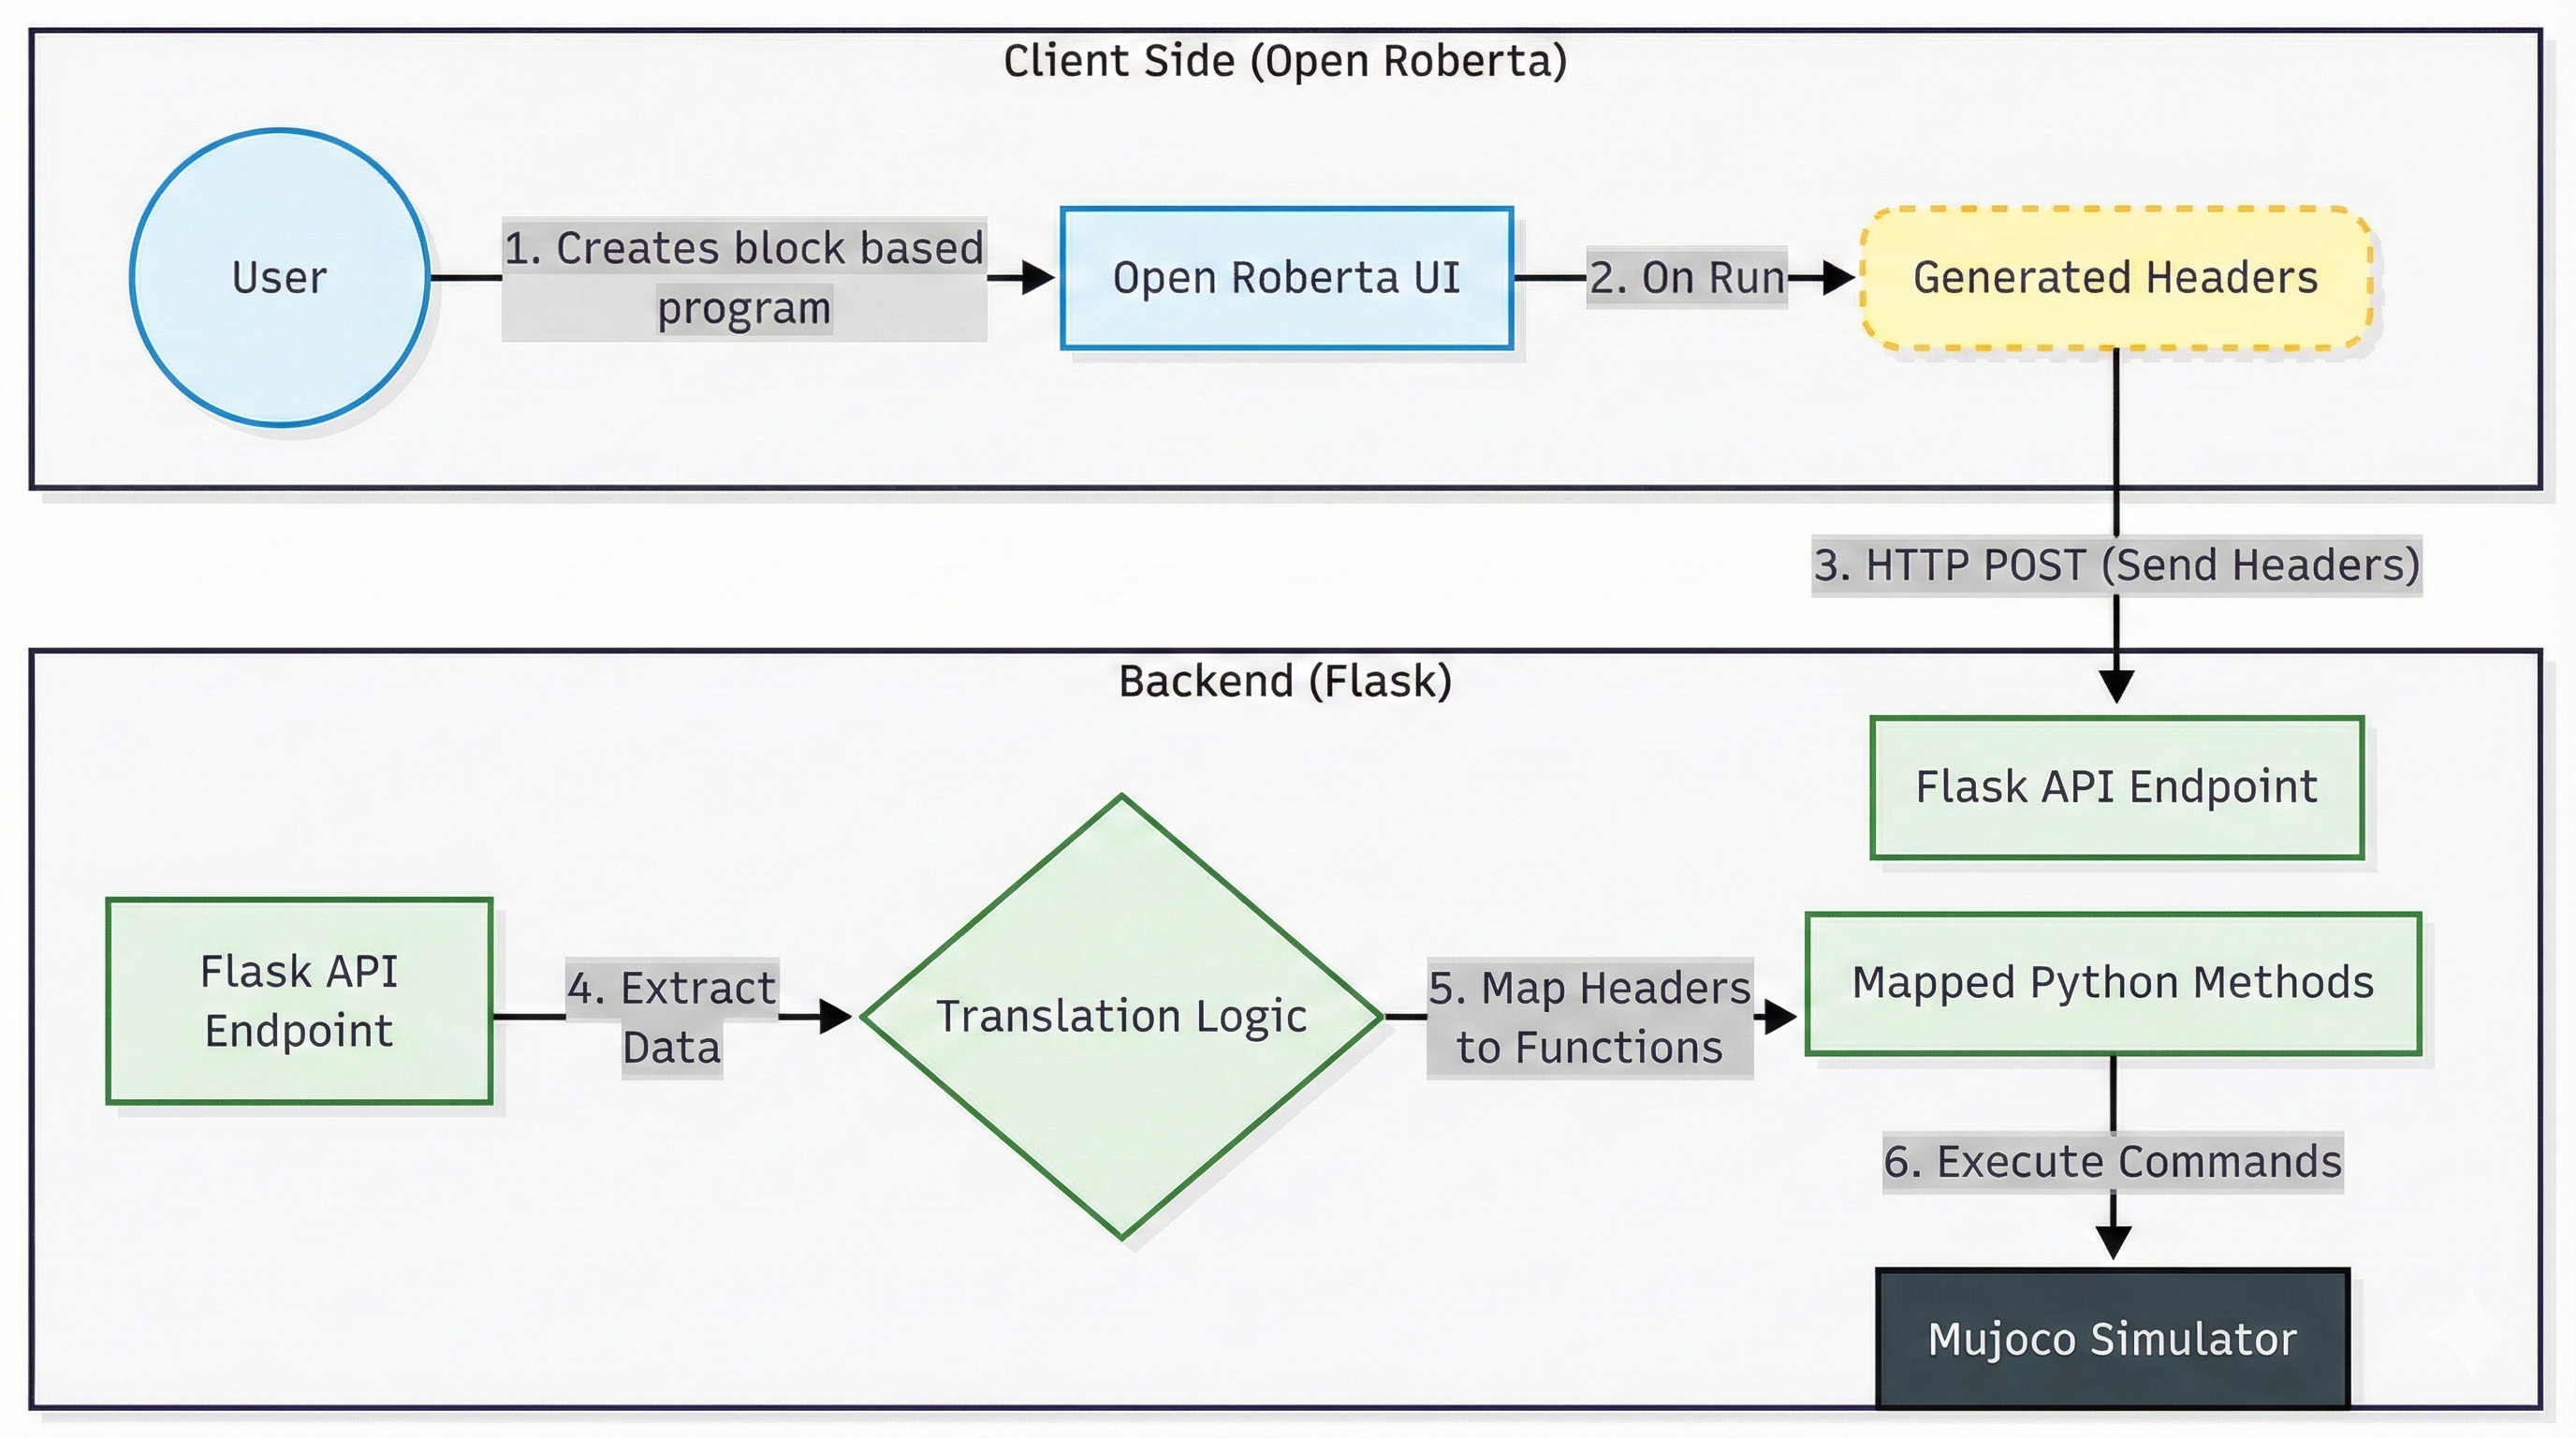
\includegraphics[height=0.9\textheight,keepaspectratio]{ArchitectureH2.png}
    \caption{System architecture}
    \label{fig:architecture-zoom}
    \Description{System architecture diagram showing the Client Side, Backend, and Simulator tiers in more detail.}
\end{figure}



\subsubsection{Detection Algorithm}
	exttt{highlightOnlyFunctionCandidates} function. The approach is intentionally simple so it is easy to read
and to implement in a real block editor. The algorithm follows three main steps:
%\begin{itemize}
 %   \item \textbf{Linearization:} Convert the workspace into a flat, ordered list of blocks (preserving execution order).
 %   \item \textbf{Identify sequences:} Slide a window over the list and extract contiguous sequences whose length is at least a minimum (e.g. 3).
 %   \item \textbf{Pattern Matching:} Use the block type sequence as a key; group occurrences with the same key and report keys seen more than once.
%\end{itemize}

\texttt{highlightOnlyFunctionCandidates} function. The algorithm operates in several steps:
\begin{itemize}


    \item \textbf{Linearization:} First, the algorithm linearizes the block workspace into a sequential list of blocks. 
    
    \item \textbf{Identify sequences:} It then iterates through this list to identify all possible sequences of blocks that meet a minimum unique block type length requirement (three blocks) that can be repeated more than once.
    
    \item \textbf{Sequences Matching:} If the same sequence of block types is found more than once, it will be added to the CustomReusableCandidates list which will eventually be sorted by longest and most recent duplicated sequences. In the end the highest priority candidate gets returned.


\end{itemize}

The pseudocode below is short, explicit, and uses straightforward data structures (lists).

\begin{algorithm}[H]
\caption{Duplicate Sequence Detection}
\label{alg:detection_refined}
\begin{algorithmic}[1]
\REQUIRE Workspace, StartBlock \quad // user's block workspace
\REQUIRE MinimumSequenceLength = 3, MinimumDifferentBlockTypesInSequence = 3, MaxSequenceLength = 10 \quad
\ENSURE ReusableComponentCandidates \quad // list of repeated block sequences to return
\STATE Chain $=$ \textbf{buildLinearChain}(StartBlock) 
\STATE Sequences $=$ List$\langle$sequence$\rangle$ 

\FOR{startIndex = 0 \TO length(Chain) - 1} 
    \FOR{$sequenceLength = 1$ \TO $MaxSequenceLength$ }
        \STATE sequence $=$ Chain[startIndex \,..\, startIndex + sequenceLength - 1] 
        \STATE numberOfBlockTypesInSequence = getNumberOfDistinctBlockTypes(sequence)
        \IF{sequenceLength >= MinimumSequenceLength \textbf{ and } numberOfBlockTypesInSequence >= MinimumDifferentBlockTypesInSequence}
            \STATE Sequences.append(sequence) // record sequence occurrence
        \ENDIF
    \ENDFOR
\ENDFOR

\STATE ReusableComponentCandidates $= \{\text{Sequences} \mid occurrence \ge 2 \}$ 
\STATE sort ReusableComponentCandidates by (longest sequence length and most recent occurrence) 
\RETURN ReusableComponentCandidates[0] // Return highest priority candidate
\end{algorithmic}
\end{algorithm}


Algorithm 1. Illustrates the core logic for identifying duplicate block sequences

%\begin{algorithm}[H]
%\caption{Highlight duplicate sequences}
%\label{alg:detection_refined}
%\begin{algorithmic}[1]
%\REQUIRE Workspace, StartBlock \quad // user's block workspace
%\STATE SequenceToHighlight = DuplicateDetectionAlgorithm()
%\FOR{each SequenceToHighlight in Workspace}
%    \FOR{block in SequenceToHighlight} 
%        \STATE block.changeColor(GREEN) \quad // highlight duplicate blocks
%        \STATE alertUser("Duplicate sequence detected. Create reusable block?")
%        \IF{userConfirms()} 
%            \STATE createReusableBlockFromSequence(block)
%        \ENDIF
%    \ENDFOR
%   \ENDFOR
%\end{algorithmic}
%\end{algorithm}
%Algorithm 2. Illustrates when the system highlights duplicate sequences and alerts the user to create reusable blocks


%\begin{algorithm}[H]
%\caption{Event Listener}
%\label{alg:detection_refined}
%\begin{algorithmic}[1]
%\REQUIRE Workspace, StartBlock \quad // user's block workspace
%\STATE Window.eventListener("onEachEvent", HighlightDuplicateSequences,ResetBlockColors)
%\end{algorithmic}
%\end{algorithm}

%Algorithm 3. Illustrates how the detection algorithm is triggered on each user event in the workspace

% [TODO: Insert here your technical description from your original section 3.2.1. 
% Explain briefly the architecture, the detection algorithm, and how the UI works.]
\subsubsection{User Interface and Interaction}
The user interface is designed to be intuitive and non-disruptive. When the detection 
algorithm identifies a candidate, the system visually highlights the blocks on the canvas as illustrated in Figure \ref{fig:ui_interaction_highlight}. 
A non-blocking toast notification appears, prompting the user to confirm the refactoring. 
If confirmed, the system automatically generates the custom block definition in a dedicated 
workspace area (handling visibility via \texttt{revealDefinitionWorkspacePane}) and updates
the main workspace, replacing the redundant code with concise function calls as shown in Figure \ref{fig:ui_interaction_refactor}. 
This process abstracts the complexity of manual function creation, guiding the user toward modular 
design practices.

% --- START: Split UI figures ---
\begin{figure}[htbp]
    \centering
    % Prefer vector PDF when available, fallback to PNG/JPG
    \includebestgraphics[width=0.85\linewidth]{highlight}
    \Description{A screenshot of the Open Roberta environment. Two identical sequences of blocks are highlighted. A pop-up message in the bottom right asks the user if they want to create a reusable block.}
    \caption{Reuse Assistant workflow — detection: the interface detects and highlights duplicate blocks by changing their color to green.}
    \label{fig:ui_interaction_highlight}
\end{figure}

\begin{figure}[htbp]
    \centering
    % Prefer vector PDF when available, fallback to PNG/JPG
    \includebestgraphics[width=0.85\linewidth]{custom_component}
    \Description{Screenshot showing the code after refactoring. The main program is now much shorter. A side panel shows the definition of the new custom block with parameters for coordinates.}
    \caption{Reuse Assistant workflow — refactoring: the automated refactoring result, showing the new custom block definition and the simplified main program.}
    \label{fig:ui_interaction_refactor}
\end{figure}
% --- END: Split UI figures ---

% Esto prohíbe que las imágenes pasen de aquí hacia abajo. 
% Se imprimirán antes de que empiece la sección 3.3 obligatoriamente.
\FloatBarrier
% -------------------------------------------------------------------------------------------------------------------------------------------------------------------
% validity threat here or in discussion?
% Treatment validation needs to be split into subsections "data gathering and analysis" How we gather the data and how we analyze them
%"Task execution" We need to explain what exactly will be the task
\subsection{Treatment Validation}
The treatment validation for this study adopts a mixed-methods evaluation approach to assess 
the effectiveness of the proposed features for guiding users in creating custom reusable components (blocks) within 
the OpenRoberta environment. 

\subsubsection{Participant Recruitment}
A total of 10 participants will be selected to ensure a diverse range of experience levels with block-based programming. 
Time constraints and resource availability have influenced the decision to limit the number of participants.
Participants will be recruited from a diverse pool of individuals affiliated with the University of Southern Denmark and the broader chemistry community. 
This group of participants includes chemistry teachers, professional chemical engineers, and students currently enrolled in chemistry-intensive curricula. 
To ensure relevant practical expertise, the selection specifically targets those who frequently engage in laboratory environments. 
The experimental sessions will be conducted across a range of environments to accommodate participant availability. 
Physical sessions will take place within the chemistry laboratories at the University of Southern Denmark (SDU) as well as a private residential setting. 
For remote participants, sessions will be administered virtually using Discord for communication and AnyDesk for remote desktop control.

\paragraph{Ethical Considerations and Sampling}
Prior to the commencement of the study, all participants are required to sign a consent form acknowledging their voluntary participation and granting permission for screen recording and data usage. 
It should be noted that this recruitment strategy constitutes \textit{convenience sampling}. As such, they may not represent the general population.
% -------------------------------------------------------------------------------------------------------------------------------------------------------------------
\subsubsection{Task Execution}
The participants will initially be given a short introduction to the OpenRoberta UI, as well as the mujoco robot simulator. 
They will then perform one task which is described by a set of pre-defined steps to perform. This task has been specifically designed to promote the reusability aspect.
The task is focused on the domain of chemistry, as it is modelled after a real lab experiment perfomed by chemistry students at SDU. 

The participants will be instructed to program the robot to execute the following sequence of operations:

\begin{enumerate}
    \item Move the robot arm above mix cylinder
    \item Mix the chemistry ingredients
    \item Move the robot arm above the analysis pad
    \item Analyze the sample
    \item If the solution is analyzed (use if statement) then show a response message in the laptop’s screen 
    \item Place the following three objects into their corresponding slots in the chemistry equipment toolbox:
    \begin{itemize}
        \item Methanol cylinder
        \item Chloroform syringe
        \item Toluene syringe
    \end{itemize}
    \item Important notes for the participants:
    \begin{itemize}
        \item \textit{After placing an object to its slot in the toolbox \textbf{wait 2 seconds} before you move to pick a new one.}
        \item \textit{After placing the \textbf{chloroform syringe} to its slot, \textbf{move the robot arm up by 10 cm} before you move to pick the next chemistry object }
        \item \textit{Click the \textbf{play} button on the bottom right corner to start the simulation}
        \item \textit{Click the \textbf{reset} button on the bottom right corner to reset the scene of the robot simulator}
    \end{itemize}
\end{enumerate}

Most optimal solution pre-defined by the researchers:
 \begin{figure}[h]
     \centering
     \includegraphics[width=0.8\textwidth]{most optimal solution.png}
     \caption{The optimal solution implemented in OpenRoberta, utilizing a custom block for the object placement sequence.}
     \Description{Block-based program showing the optimal solution with a custom reusable block for placing chemistry objects into toolbox slots.}
     \label{fig:optimal_solution}
 \end{figure}

Instead of creating a long linear sequence of blocks (hard-coding the movement for all three objects), the most optimal solution utilizes a **Custom Reusable Component** to handle the repetitive action of placing an object to its corresponding slot inside the equipment toolbox. 
This approach not only reduces redundancy but also enhances code maintainability and readability, aligning with best practices in software development.

All the participants will try to complete the task using both the standard and the enhanced version of OpenRoberta. 
Half of the participants will begin using the enhanced version of OpenRoberta, while the other half will start with the standard version.
Participants’ interactions with the platform will be observed throughout the task.
Guidance will be provided from the researchers to the participants throughout the task.

% -------------------------------------------------------------------------------------------------------------------------------------------------------------------
\subsubsection{Data Gathering and Analysis}
Data collection focuses on both quantitative performance and qualitative feedback from participants:
\begin{enumerate}
    \item \textbf{Task Completion Time:} Comparing the participants who will first use the enhanced version of OpenRoberta against those who will first use the standard version.
    \item \textbf{Solution Accuracy:} Evaluated by comparing the participant's block configuration against the pre-defined optimal solution.
    \item \textbf{Survey Feedback:} Collected via a post-experiment survey designed to capture demographic data and subjective perceptions of the utility of the block creation guidance features.
\end{enumerate}

This comprehensive evaluation will provide a detailed understanding of how useful and effective is the block creation guidance feature to the end-users.
%-------------------------------------------------------------------------------------------------------------------------------------------------------------------
\section{Results}
% -----------------------------------------------------------------------------------------
% OVERVIEW
% -----------------------------------------------------------------------------------------
The treatment validation was concluded with a total of 10 participants. 
The analysis of the collected data combines quantitative metrics regarding user preference and satisfaction 
with qualitative feedback derived from survey responses.


\subsection{Performance Evaluation}
To evaluate the efficiency and effectiveness of the proposed reusable component features, 
we analyzed two primary metrics: Task Completion Time and Solution Accuracy.

% -----------------------------------------------------------------------------------------
% TASK COMPLETION TIME
% -----------------------------------------------------------------------------------------
\subsubsection{Task Completion Time}
The total time required to complete the experimental task was recorded for both the \textit{Standard} and \textit{Enhanced} conditions. 

We compared the performance of participants based on the order of conditions (see Table \ref{tab:time_comparison_vertical}).
The analysis reveals a significant reduction in task duration when using the Enhanced 
version. The average completion time for the participants that used the Enhanced version first was $8.5$ 
minutes, compared to $10$ minutes for the Standard version. 
\begin{equation}
    \text{Efficiency Improvement} = \frac{10.0 - 8.5}{10.0} \times 100\% = 15\%
\end{equation} 



%\begin{itemize}
 %   \item \textbf{Enhanced OpenRoberta version First:} Participants who started with the Enhanced version completed the task in an average of 8 and a half minutes.
 %   \item \textbf{Standard OpenRoberta version First:} Participants who started with the Standard version completed the task in an average of 10 minutes.
%\end{itemize}
\begin{table}[h]
    \centering
    \caption{Breakdown of Mean Task Completion Times}
    \label{tab:time_comparison_vertical}
    % 'm{10cm}' allows the text to wrap and centers it vertically
    % 'c' centers the number vertically
    \begin{tabular}{m{10cm} | c} 
        \hline
        \textbf{Experimental Condition} & \textbf{Mean Time (min)} \\
        \hline
        % No '\\' here. Text and number are on the same row.
        \textit{Group of Participants that used the Enhanced OpenRoberta Version First} & 8.5 \\
        \hline
        \textit{Group of Participants that used the Standard OpenRoberta Version First} & 10.0 \\
        \hline
    \end{tabular}
\end{table}

% -----------------------------------------------------------------------------------------
% SOLUTION ACCURACY 
% -----------------------------------------------------------------------------------------
\subsubsection{Solution Accuracy}
Solution accuracy was evaluated by comparing participant solutions against the optimal reference 
solution defined in the treatment evaluation.

\paragraph{Adoption of Reusable Blocks}
A key metric was the voluntary adoption of the custom reusable component. 
In the \textit{Enhanced} version, $10/10$ participants successfully implemented a custom reusable block to handle the repetitive object placement steps. 
In contrast, in the \textit{Standard} condition, participants predominantly relied on linear, repetitive code structures.
Without the guidance features, none of them recognized the opportunity to create a reusable block.

% -----------------------------------------------------------------------------------------
% SURVEY QUANTITATIVE RESULTS
% -----------------------------------------------------------------------------------------
\subsection{Survey Quantitative Results}

\subsubsection{User preference between Standard and Enhanced Versions of OpenRoberta}
The survey results indicate a unanimous preference for the enhanced version of the OpenRoberta Lab. 
As illustrated in Figure \ref{fig:compare_versions}, 70\% of participants rated the enhanced version 
as ``much better'' than the standard version, while the remaining 30\% rated it as ``better.'' 
No participants preferred the standard version or rated the two versions as equivalent.

\begin{figure}[h]
    \centering
    % Use PDF (vector) if present, otherwise PNG/JPG
    \includebestgraphics[width=\textwidth]{survey_comp_enh_sta}
    \caption{Summary of participant responses regarding overall preference between the standard and enhanced versions of OpenRoberta}
    \label{fig:compare_versions}
\end{figure}
\begin{figure}[h]
    \centering
    \includebestgraphics[width=\textwidth]{usability_of_feature}
    \caption{Summary of participant responses regarding overall preference between the standard and enhanced versions of OpenRoberta}
    \label{fig:usability_of_feature}
\end{figure}
\begin{figure}[h]
    \centering
    \includebestgraphics[width=\textwidth]{hl_eval}
    \caption{Summary of participant responses regarding overall preference between the standard and enhanced versions of OpenRoberta}
    \label{fig:hl_eval}
\end{figure}
\begin{figure}[h]
    \centering
    \includebestgraphics[width=\textwidth]{hl_pref}
    \caption{Summary of participant responses regarding overall preference between the standard and enhanced versions of OpenRoberta}
    \label{fig:hl_pref}
\end{figure}

\subsubsection{Usability of the Guidance Feature}
Regarding usability of the enhanced OpenRoberta version, we received high acceptance scores. As illustrated in Figure \ref{fig:usability_of_feature}, 40\% of participants found the 
enhanced version ``very easy'' to use, and 60\% rated it as ``easy.''
No participants rated the enhanced version as ``Neither easy nor difficult,'' ``Difficult,'' or ``Very difficult'' to use.
\subsubsection{Evaluation of the Visual Highlighting}
A key component of the enhanced version was the visual highlighting designed 
to guide the user into an automatic custom reusable block creation. 
As shown in Figure \ref{fig:hl_eval}, results showed a high level of user satisfaction, with 90\% of participants reporting they were either ``satisfied'' 
(20\%) or ``very satisfied'' (70\%) with the features. Only one participant (10\%) expressed a neutral stance.

\subsubsection{Visual Highlighting Style Preference}
When asked about specific highlighting preferences, as depicted in Figure \ref{fig:hl_pref} the \textit{Animated Color Highlight} was the most popular choice, 
preferred by 50\% of the users. A significant portion of participants (30\%) expressed no strong preference 
between the styles, suggesting that the presence of guidance was more important than the specific animation style 
used.

% -----------------------------------------------------------------------------------------
% SURVEY QUALITATIVE RESULTS
% -----------------------------------------------------------------------------------------
\subsection{Qualitative Feedback}
The post-experiment survey included open-ended questions to gather detailed feedback. The thematic analysis of 
these responses revealed two primary findings:

\paragraph{Efficiency and Speed}
When asked to identify the biggest difference between the two versions, the majority of participants cited 
\textit{efficiency}. Responses frequently described the enhanced version as ``faster'' and noted that it 
``saved a lot of time.'' This aligns with the quantitative preference data, suggesting that the reusability 
features successfully reduced the perceived workload.

\paragraph{Suggestions for Improvement}
Participants also provided constructive feedback regarding the function blocks. Two participants specifically 
suggested that the system should more clearly \textit{``specify parameter names''} within the function blocks to 
improve clarity. Another participant noted that the function call block should be pre-configured for immediate 
use in the blockchain. These suggestions highlight a need for clearer labeling in future iterations of the 
interface.

%----------------------------------------------------------------------------------------------------------------------
\section{Discussion}
%In this section, you should discuss the results presented in the previous section. The discussion should be organized around lessons learned (5.1), implications for practice (5.2), and threats to validity (5.3). The whole discussion must be grounded on the existing literature and argue how your contributions advance the state-of-the-art in the chosen EUSE area
%need to review the screen recordings as well!! How was the users' behavior when using the enhanced tool? How long does it take them to insert a custom block into the workflow, after they've clicked 'yes' to letting our tool create one for them? Did they seem confused or hesitant when they used the tool for the first time?
% Another thing we should refine in section 3 - we should prolly explain more about why we designed the tool the way we did. Need to back it up with research. 

\subsection{Lessons Learned}
Utilizing OpenRoberta Lab as a representative block-based robotics environment, this study examined the 
efficacy of automated guidance mechanisms in promoting software reuse among chemistry students and educators 
engaged in laboratory experimentation.


Based on the feedback from the participants, as well as observations of how they solved the task, 
the participants found the enhanced version of OpenRoberta Lab to be better than the standard version. 
Noteably, 9 out of 10 participants commented on how the enhanced version let them perform their task faster. 
As described in section 2, this is also one of the main benefits of reuse in the field of software engineering. 

\subsubsection{Overcoming the Recognition Barrier for Reuse}
A defining finding of this study is the contrast in adoption rates: 100\% of participants utilized 
reusable blocks in the \textit{Enhanced} version of OpenRoberta Lab, compared to 0\% in the \textit{Standard}. 
This confirms the literature cited in Section 1 regarding the high barrier to entry for "Citizen Developers". 
Despite the task being repetitive by design, participants in the standard environment prioritized immediate 
task completion over code optimization (linear programming). The \textit{Enhanced} version successfully 
shifted this behavior not by forcing reuse, but by lowering the cognitive cost of identifying opportunities. 
This suggests that for domain experts like chemists, the barrier to reuse is not a lack of utility, but a 
lack of recognition.

\subsubsection{Impact of Automated Construction of Reusable Components} 
The 15\% reduction in task completion time highlights the value 
of automating the block creation process. In the standard environment, creating a reusable component requires
a manual, multi-step process of defining a function and relocating blocks. The enhanced version streamlined 
this by automating the structural setup of the custom block once a duplicate was detected. This confirms that 
removing the "friction" of manual block assembly is crucial for encouraging reusability among non-programmers.

\subsubsection{Visual Salience in Learning}
The user preference for the \textit{Animated Color Highlight} (50\% preference) and the high satisfaction 
rates (90\% satisfied/very satisfied) underscore the importance of visual salience. In a dense visual 
environment like OpenRoberta, static cues are easily overlooked. The dynamic nature of the animation acted 
as a "Just-in-Time" trigger, interrupting the user's tunnel vision exactly when the redundancy occurred. 
This supports the use of proactive, visually distinct interruptions in educational IDEs to correct inefficient
patterns in real-time.

\subsubsection{Suggestions by Participants}
Changes suggested by the participants mainly focus on smaller customizations of the tool and the OpenRoberta 
Lab UI. It would be amiss to claim that the lack of suggested changes, focused on the tool overall, indicate 
that there is no need for improvement of the tool. As many of the participants consider themselves 'beginners'
in regards to Computer Programming, it's likely that they lack ideas about other ways the tool could have been 
designed. Instead, these answers can be interpreted as the participants having little to no issue with the 
current design. 

\subsection{Implications for Practice}
% From what I could find, this section is basically about the potential effects/significance of our study's findings. How can the results we found influence real-life practices and research? Basically smth like; participants showed positive reactions to our tool, finding it both easier to use, but also faster. Our solution/idea is worth doing further research about, as the results suggest that our idea can successfully help end-users perform reuse. 
The findings of this study have broader implications for the design of End-User Development (EUD) environments 
and educational technology. The success of the enhanced OpenRoberta interface suggests three key shifts for 
future tool development:

\subsubsection{Transitioning from Passive to Proactive Environments}
Current block-based environments (such as Scratch or standard OpenRoberta) largely rely on a \textit{passive} 
interaction model, where advanced features like "Functions" sit in a toolbox waiting to be discovered. 
Our study demonstrates that domain experts (e.g., chemists) often fail to utilize these features voluntarily, 
even when they would be beneficial. The 100\% adoption rate in the Enhanced condition implies that EUD tools 
must evolve into \textit{active assistants}. Development environments should incorporate background monitoring
systems that detect inefficient patterns (such as code duplication) and proactively intervene with 
architectural suggestions.

\subsubsection{Learning by Example}
Beyond just making the task faster, the tool also acted as a teaching aid. By pointing out the repetitive 
code and showing how to fix it, the tool created a "learning moment" exactly when the user needed it. 
This suggests that automation tools can have two benefits: they help experts work faster, but they also teach 
beginners difficult concepts—like how to organize blocks of code and use inputs—simply by showing them a 
practical example.

\subsection{Threats to Validity}
\subsubsection{Convenience Sampling} 
The participants to the study were either aquantiances of one of the authors of the study, or were recruited 
through these aquantiances. As such, the results of this study do not represent the general population within 
the domain of chemistry. 
\subsubsection{Limitations to observation} 
Due to constraints with time and flexibility, only one of the authors was present to observe the participants. 
To ensure that data from the observation was not affected by this, a screen recording of each participant 
performing the task was saved. Several of the authors reviewed and discussed these recordings together to 
extract data.





\section{Appendices}

If your work needs an appendix, add it before the
``\verb|\end{document}|'' command at the conclusion of your source
document.

Start the appendix with the ``\verb|appendix|'' command:
\begin{verbatim}
  \appendix
\end{verbatim}
and note that in the appendix, sections are lettered, not
numbered. This document has two appendices, demonstrating the section
and subsection identification method.





%%
%% The next two lines define the bibliography style to be used, and
%% the bibliography file.
\bibliographystyle{ACM-Reference-Format}
\bibliography{sample-base}


%%
%% If your work has an appendix, this is the place to put it.
\appendix


\end{document}
\endinput
%%
%% End of file `sample-manuscript.tex'.
